% We import package amsmath before the documentclass to avoid the warning.
% Command '\usepackage{amsmath}' results in the following warning:
% Package amsmath Warning: Unable to redefine math accent \vec.
\RequirePackage{amsmath} % for environments such as align

\documentclass[runningheads]{llncs}

% If possible, figure files should be included in EPS format.

% If you use the hyperref package, please uncomment the following two lines
% to display URLs in blue roman font according to Springer's eBook style:
%\usepackage{color}
%\renewcommand\UrlFont{\color{blue}\rmfamily}

% The following code is used to remove the warning with subcaption package:
% ------------------------------
% Package caption Warning: Unknown document class (or package),
% standard defaults will be used.
% ------------------------------
% cf. https://teratail.com/questions/q2vuwf6skm5hph
\makeatletter
\def\caption@documentclass{elsarticle}
\makeatother

\usepackage[export]{adjustbox} % for valign option in \includegraphics
\usepackage{algorithm}
\usepackage{algpseudocode}
\usepackage{amssymb} % for \mathbb
\usepackage{array} % for m column type
\usepackage{bbm} % for \mathbbm
\usepackage{booktabs} % for \toprule, \midrule, \bottomrule
\usepackage{cleveref} % for \cref
\usepackage{color,soul} % for \hl
\usepackage{csvsimple} % for \csvreader
\usepackage[T1]{fontenc} % for T1 font encoding
\usepackage{graphicx} % for \includegraphics
\usepackage{pgffor} % for \foreach
\usepackage[labelformat=simple]{subcaption} % for subfigure environment
\usepackage{tikz}
\usetikzlibrary{positioning}

% The following code is used to remove the warning with bibliography:
% ------------------------------
% Underfull \hbox (badness 2653) in paragraph at lines 28--34
% ------------------------------
% cf. https://tex.stackexchange.com/questions/10924/underfull-hbox-in-bibliography
\apptocmd{\sloppy}{\hbadness10000\relax}{}{}

% set the path for figures
\graphicspath{{./src/img}{./src/experiments}}

% set the label format for subcaption
\renewcommand\thesubfigure{(\alph{subfigure})}

% settings for cleveref
\crefname{table}{Table}{Tables}
\crefname{algorithm}{Algorithm}{Algorithms}
\crefname{figure}{Fig.}{Figs.}

% import the TeX file containing macro definitions
\newcommand{\ispace}{\mathbb{D}^{m}}
\newcommand{\Prec}{\operatorname{acc}}
\newcommand{\Cov}{\operatorname{cov}}
\newcommand{\cands}{\bar{\mathcal{A}}}
\algnewcommand{\IIf}[1]{\State\algorithmicif\ #1\ \algorithmicthen\ }
\renewcommand{\algorithmicrequire}{\textbf{Input:}}
\renewcommand{\algorithmicensure}{\textbf{Output:}}


% TODO REBUTTAL: Please enter paper ID
\def\paperID{735} % *** Enter the paper ID here


\begin{document}
\begin{center}
  % smaller title font only for rebuttal
  % additional two empty lines at the end of the title
  \vspace*{-22pt}
  \begin{tabular}[t]{c}{
      \large\bf
      Paper ID \paperID{}
    }
  \end{tabular}
  \par
  % additional small space at the end of the author name
  % additional empty line at the end of the title block
\end{center}
We deeply appriciate all the reviewers who made sharp and valuable comments
on our paper and gave us the opportunity to submit a revised version.
We have done our best for the revision according to their comments as shown below.
We also would like to thank in advance all the reviewers for reconsidering
the suitability of our revised paper for the conference.

\section*{Summary of revisions}
We would like to appriciate all the reviewers for their clear and insightful
comments.
We improved our paper from the original version according to their comments.
The major revision points are listed as follows:
\begin{enumerate}
  \item We added an overview of other existing methods in \cref{sec:related-work}.
  \item We added discussion about parameter selection in \cref{sec:param}.
  \item We conducted qualitative and quantitative comparisons
        between Anchor and R-LIME in \cref{sec:exp-qual,sec:exp-anchor}.
\end{enumerate}
Please see below for a point-by-point response to each reviewer's comments.

\newenvironment{mycomment}{
  \vspace{10pt}\hspace{.02\textwidth}\begin{minipage}{.92\textwidth}
    }{\end{minipage}}

\section*{Responding to Reviewer \#1}
Suggestions for Rebuttal:
\begin{enumerate}
  \setlength{\itemsep}{15pt}
  \item Offer guidance on how to select optimal parameters for different
        datasets and models.

        \begin{mycomment}
          We would appreciate for your suggestion.
          We added \cref{sec:param} as a guidance on how parameters should be
          selected in practice.
        \end{mycomment}

  \item Include a discussion of other model-agnostic interpretability methods,
        such as SHAP, to provide a more comprehensive overview.

        \begin{mycomment}
          Thank you for your valuable suggestion.
          We should add an overview of other model-agnostic interpretability
          methods, but we only added names of some other methods to
          \cref{sec:related-work}, because of lack of space.
        \end{mycomment}

  \item Add experimental comparisons with more other model-agnostic \\
        interpretability methods to better evaluate R-LIME's effectiveness.

        \begin{mycomment}
          We would like to appriciate your sharp observations.
          We additionally conducted qualitative and quantitative comparisons
          between Anchor and R-LIME,
          which demonstrated that R-LIME generates more informative and
          general explanations than Anchor (see \cref{sec:exp-qual,sec:exp-anchor}).
        \end{mycomment}
\end{enumerate}
\section*{Responding to Reviewer \#4}
The authors should kindly explain why there is not a quantitative comparison
between their proposed method R-LIME and Anchor. The lack of the comparison
makes it hard to evaluate the impact of the proposed model.

\begin{mycomment}
  We would appreciate for your insightful comments.
  We additionally conducted qualitative and quantitative comparisons
  between Anchor and R-LIME,
  which demonstrated that R-LIME generates more informative and
  general explanations than Anchor (see \cref{sec:exp-qual,sec:exp-anchor}).
\end{mycomment}

\section*{Responding to Reviewer \#5}
\begin{itemize}
  \setlength{\itemsep}{15pt}
  \item It would be beneficial to move the comparison of R-LIME with Anchor
        and LIME to the Related Work section for improved clarity and
        organization.

        \begin{mycomment}
          We would like to appriciate for your insightful suggestion.
          We interpreted your suggestrion to mean that we should move
          \cref{fig:example} and its explanation to \cref{sec:related-work}.
          We discussed about the most understandable structure of our paper.
          And for clarity, we concluded that we should present effectiveness
          of R-LIME compared to existing methods closely related to our method
          in \cref{sec:introduction},
          before we overview other existing methods in \cref{sec:related-work}.
        \end{mycomment}

  \item The authors should consider exploring a more compatible method than the
        KL-LUCB algorithm to achieve higher accuracy. Although the experimental
        results suggest a minor effect, there may be potential underlying issues
        that need to be addressed.

        \begin{mycomment}
          Thank you for your valuable feedback.
          It is true that we must address theoretical issues for using
          KL-LUCB algorithm, although our results suggest that its practical
          effect is negligible.
          We focus on presenting our novel framework for local interpretability,
          not on the detailed algorithm.
          Thus, we leave the issues for future work because of lack of space.
          But we deeply appreciate for your sharp observations.
        \end{mycomment}

  \item The title of the `Challenges and Future Work' section could be more
        aptly replaced with `Discussion' to better reflect the content.

        \begin{mycomment}
          Thank you for your suggestion. We renamed the section to `Discussion'
          for clearly reflecting the content.
        \end{mycomment}
\end{itemize}

\newcommand{\sampleindex}[1]{\ifnum#1=0 \Asample\else\Bsample\fi}
\def\AB#1{\ifnum#1=0 A\else B\fi}

\def\paper{

% The title of the paper
\title{%
  R-LIME\@: Rectangular Constraints and Optimization for Local Interpretable
  Model-agnostic Explanation Methods
}

% Abbreviated title for the running head
\titlerunning{%
  R-LIME\@: Rectangular Constraints and Optimization for LIME Methods
}

% Author names and ORCID IDs
\author{Genji Ohara\orcidID{0009-0000-5854-2820} \and % chktex 8
  Keigo Kimura\orcidID{0000-0002-3614-6568} \and      % chktex 8
  Mineichi Kudo\orcidID{0000-0003-1013-3870}          % chktex 8
}

% Abbreviated author list for the running head (First names are abbreviated)
% If there are more than two authors, 'et al.' is used.
\authorrunning{G. Ohara et al.}

% The authors' affiliations
\institute{Division of Computer Science and Information Technology\\
  Graduate School of Information Sci.\ and Tech.,
  Hokkaido University\\
  Sapporo 060--0814, JAPAN,\\
  \email{\{genji-ohara, kimura5, mine\}@ist.hokudai.ac.jp}}

\maketitle

% The abstract should briefly summarize the contents of the paper in
% 150--250 words.
\begin{abstract}
  In recent years,
  complex machine learning models have been introduced
  in various industrial fields due to their high accuracy.
  However,
  their increasing complexity has been a major obstacle to implementation
  in sensitive decision-making situations.
  In order to address this problem,
  various post-hoc explanation methods have been proposed,
  but they have not been able to achieve interpretability of
  both the explanation and its scope.
  We propose a new method, R-LIME,
  which interprets a complex classifier in an interpretable scope.
  R-LIME locally and linearly approximates a complex decision boundary
  of a black-box classifier in a rectangular region
  and maximizes the region as long as the approximation accuracy
  exceeds a given threshold.
  The resulting rectangular region is interpretable for users because it is
  expressed as a conjunction of feature predicates.
  Through qualitative and quantitative comparisons with the existing method
  on a real-world dataset,
  we demonstrate that R-LIME provides more reliable and interpretable
  explanations than existing methods.
  % 153 words
  \keywords{Interpretable machine learning \and Local surrogate model}
\end{abstract}

\section{Introduction}\label{sec:introduction}
In recent years,
complex machine learning models, such as deep neural networks and random forests,
have been widely introduced in various industrial fields
due to their significant improvement in accuracy.
However,
their increasing complexity and black-box nature pose challenges,
particularly in critical decision-making scenarios such as healthcare and finance,
where the opacity of decision process becomes a major obstacle to implementation.
In order to address this problem,
there has been extensive research in the field of post-hoc explanations
for machine learning models
~\cite{guidotti2018local,ribeiro2016why,ribeiro2018anchors}.
Existing post-hoc explanation methods are categorized
into \emph{model-dependent} and \emph{model-agnostic} methods
based on their dependence on the model's structure,
and the latter are further classified into \emph{global} and \emph{local} methods
based on their locality in input space~\cite{samek2021explaining}.
\begin{figure}[tbp]
  \def\scale{0.38}
  \centering
  \begin{subfigure}[t]{0.55\textwidth}
    \centering
    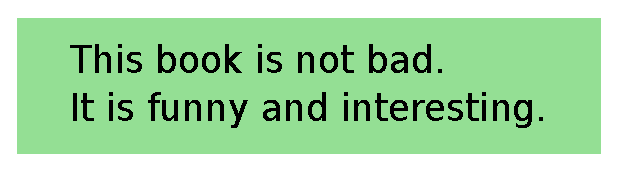
\includegraphics[scale=\scale]{example-instance}
    \caption{Focal point.}\label{fig:example-instance}
    \vspace{0.5cm}
  \end{subfigure}
  \begin{subfigure}[t]{0.45\textwidth}
    \begin{subfigure}[t]{\textwidth}
      \centering
      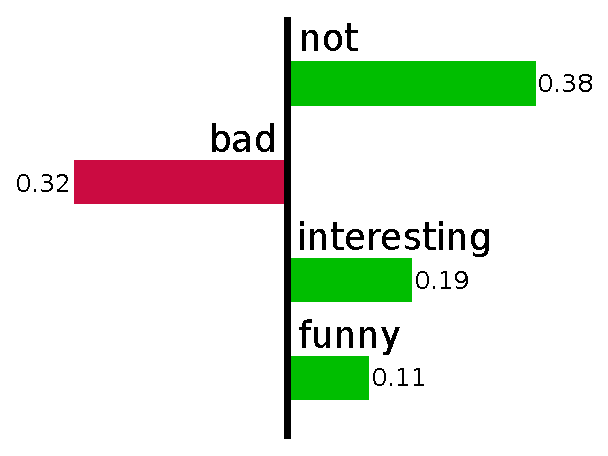
\includegraphics[scale=\scale]{example-lime}
      \caption{%
        Explanation by LIME\@.
        It provides contributions of each feature to the output,
        but does not explicitly indicate its scope.
      }\label{fig:example-lime}
      \vspace{0.4cm}
    \end{subfigure}
    \begin{subfigure}[t]{\textwidth}
      \centering
      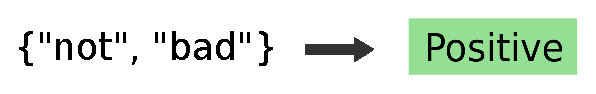
\includegraphics[scale=\scale]{example-anchor}
      \caption{%
        Explanation by Anchor.
        It provides the effective scope of the explanation,
        but does not show the influence of each feature.
      }\label{fig:example-anchor}
    \end{subfigure}
  \end{subfigure}
  \hspace{0.3cm}
  \begin{subfigure}[t]{0.45\textwidth}
    \centering
    \vspace{-2.24cm}
    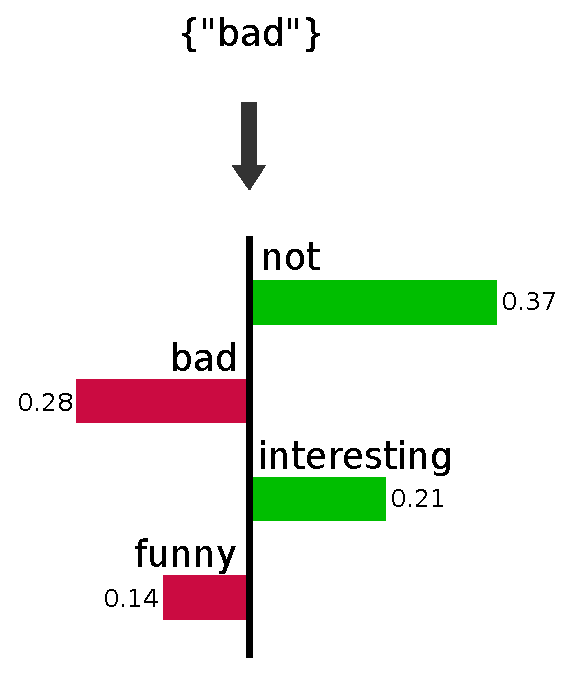
\includegraphics[scale=\scale]{example-rlime}
    \caption{%
      Explanation by R-LIME\@.
      It provides both contributions of each feature and
      its effective scope.
    }\label{fig:example-rlime}
  \end{subfigure}
  \caption[Example of explanations by LIME, Anchor and R-LIME]{%
    Example of explanations by LIME~\cite{ribeiro2016why},
    Anchor~\cite{ribeiro2018anchors} and R-LIME (our proposed method)
    for a sentiment prediction model.
  }\label{fig:example}
\end{figure}

In this paper,
we focus on \emph{local} and \emph{model-agnostic} methods.
LIME~\cite{ribeiro2016why} and Anchor~\cite{ribeiro2018anchors}
are representative local model-agnostic methods.
An example of explanations by LIME and Anchor
for a sentiment prediction model is illustrated in \cref{fig:example}.
LIME linearly approximates the complex decision boundary
around the given focal point (\cref{fig:example-instance}),
then provides the weights of the linear model as the contribution of each feature
to the output.
The explanation by LIME (\cref{fig:example-lime}) suggests that
the word ``not'' mainly contributes to the positive prediction,
but does not explicitly indicate its effective scope.
Without the scope,
users might mistakenly apply the knowledge derived from the explanation
to other instances far from the focal point,
potentially leading to misunderstanding of the black-box model's behavior
~\cite{ribeiro2018anchors}.
For this example,
users may apply the derived insights
to the sentence ``This book is not good.'' % chktex 38
and mistakenly conclude that the word ``not''
mainly contributes to the positive prediction for this sentence as well,
which is obviously incorrect.
Anchor maximizes the coverage of a rectangular region containing the focal point
as long as the probability of the black-box classifier outputting
the same label as the focal point within the region exceeds a given threshold.
While Anchor provides an effective scope of the explanation,
users can get less insight compared to LIME\@.
The explanation by Anchor (\cref{fig:example-anchor})
suggests that replacing words other than ``not'' and ``bad''
has little impact on the classifier's output.
While it clearly cannot be applied to the sentence ``This book is not good''
because of not including the word ``bad'',
the explanation does not provide details about the influence of each word,
resulting in less user insight into the model's behavior compared to LIME\@.

To address these limitations,
we propose a new method called R-LIME (Ruled LIME),
which provides both the contributions of each feature to the output
and the effective scope of the explanation.
R-LIME linearly approximates a complex decision boundary
in a rectangular region and maximizes the region
as long as the accuracy of the linear classifier exceeds a given threshold.
The region is interpretable for users because it is
expressed as a conjunction of feature predicates.
An example of the explanation by R-LIME for a sentiment prediction model
is shown in \cref{fig:example-rlime}.
It is clear that users can apply the insights derived from the explanation
only to the sentences containing the word ``not''.

\section{Related Work}\label{sec:related-work}
\begin{figure}[tbp]
  \centering
  \def\w{2.5}
  \def\ww{5.0}
  \def\h{0.5}
  \def\hh{1.3}
  \def\hhh{1.8}
  \def\hhhh{2.6}
  \begin{tikzpicture}[scale=0.9,nodestyle/.style={rectangle,auto}]
    \node[nodestyle] (post-hoc) at (0,0){post-hoc};
    \node[nodestyle] (dependent) at (-\w,-\hh){%
      \begin{tabular}{c}
        model-dependent \\
        (DTD~\cite{montavon2017explaining}, LRP~\cite{bach2015pixel})
      \end{tabular}
    };
    \node[nodestyle] (agnostic) at (\w,-\hh){\textbf{model-agnostic}};
    \node[nodestyle] (global) at (0,-\hhhh){%
      \begin{tabular}{c}
        global \\
        (PDP~\cite{friedman2001greedy}, ALE~\cite{apley2020visualizing})
      \end{tabular}
    };
    \node[nodestyle] (local) at (\ww,-\hhhh){%
      \begin{tabular}{c}
        \textbf{local} \\
        (LIME~\cite{ribeiro2016why}, Anchor~\cite{ribeiro2018anchors}, \underline{R-LIME})
      \end{tabular}
    };
    \draw(post-hoc) -- (0,-\h);
    \draw(dependent) -- (-\w,-\h) -- (\w,-\h) -- (agnostic);
    \draw(agnostic) -- (\w,-\hhh);
    \draw(global) -- (0,-\hhh)  -- (\ww,-\hhh) -- (local);
  \end{tikzpicture}
  \caption{%
    Categorization of post-hoc explanation methods.
    We focus on \emph{model-agnostic} and \emph{local} methods,
    which explain model's local behavior using only its output.
  }\label{fig:post-hoc}
\end{figure}
In this section,
we overview existing research on post-hoc explanation methods,
which explain the behavior of black-box models already trained.
As shown in \cref{fig:post-hoc},
post-hoc methods are classified into several categories.

They are broadly divided into
\emph{model-dependent} and \emph{model-agnostic} methods
based on their dependence on the model's structure.
Model-dependent methods,
such as deep Taylor decomposition (DTD)~\cite{montavon2017explaining}
and layer-wise relevance propagation (LRP)~\cite{bach2015pixel},
most of which focus on neural networks and
explain the model's behavior using its parameters~\cite{samek2021explaining}.
While these methods provide detailed explanations
(e.g., layer-wise explanations for neural networks),
it is often challenging
to apply the same method to models with different structures.
In contrast,
model-agnostic methods use only the model's output.
Although they are applicable to any model,
they cannot explain the reasoning process inside the model.

Furthermore, model-agnostic methods are categorized into
\emph{global} and \emph{local} methods based on their locality in input space.
Global methods,
such as partial dependence plots (PDP)~\cite{friedman2001greedy}
and accumulated local effects (ALE)~\cite{apley2020visualizing},
aim to explain the model's behavior across the entire input space.
However, providing global explanations becomes challenging
as the model's complexity increases.
In contrast, local methods,
such as \hl{indivisual conditional expectation (ICE)}~\cite{goldstein2015peeking},
local interpretable model-agnostic explanations
(LIME)~\cite{ribeiro2016why}, Anchor~\cite{ribeiro2018anchors} and
\hl{shapley additive explanations (SHAP)}~\cite{lundberg2017unified},
explain model's behavior in the vicinity of a specific input.
While they offer explanations more simple and accurate
than global methods,
the scope of the explanation is limited locally.

\section{Proposed Method}
\begin{figure}[tbp]
  \centering
  \begin{subfigure}[t]{0.3\textwidth}
    \centering
    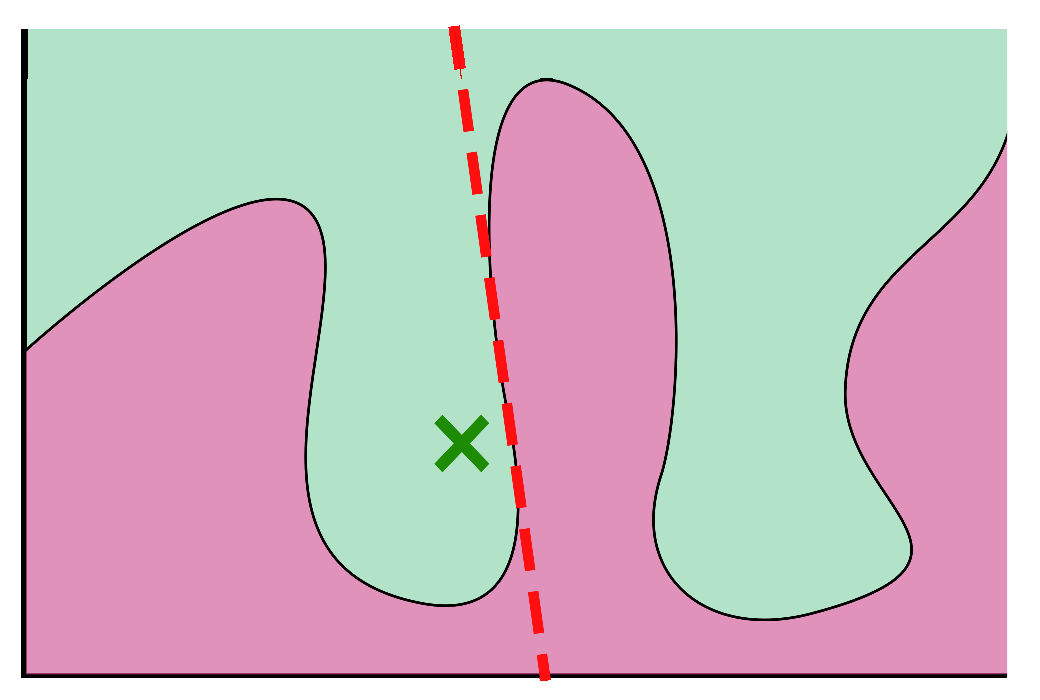
\includegraphics[width=\textwidth]{visual-lime}
    \caption{%
      LIME\@: Locally approximates the decision boundary around the focal point.
    }\label{fig:lime}
  \end{subfigure}%
  \hspace{0.03\textwidth}
  \begin{subfigure}[t]{0.3\textwidth}
    \centering
    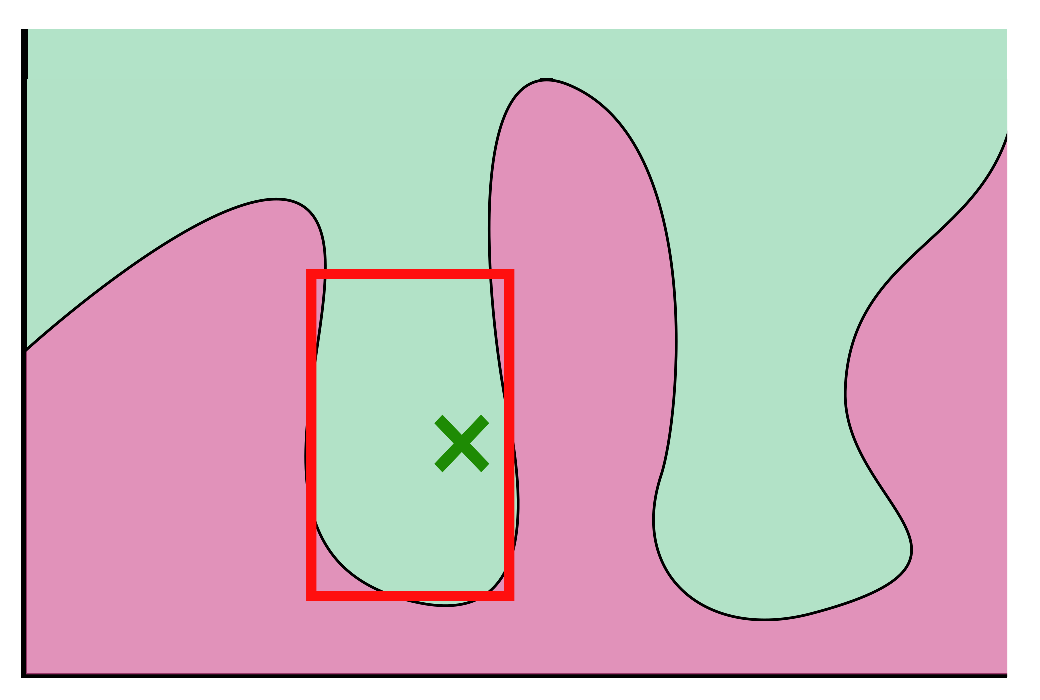
\includegraphics[width=\textwidth]{visual-anchor}
    \caption{%
      Anchor: Maximizes coverage of a rectangular region
      containing the focal point under accuracy constraints.
    }\label{fig:anchor}
  \end{subfigure}
  \hspace{0.03\textwidth}
  \begin{subfigure}[t]{0.3\textwidth}
    \centering
    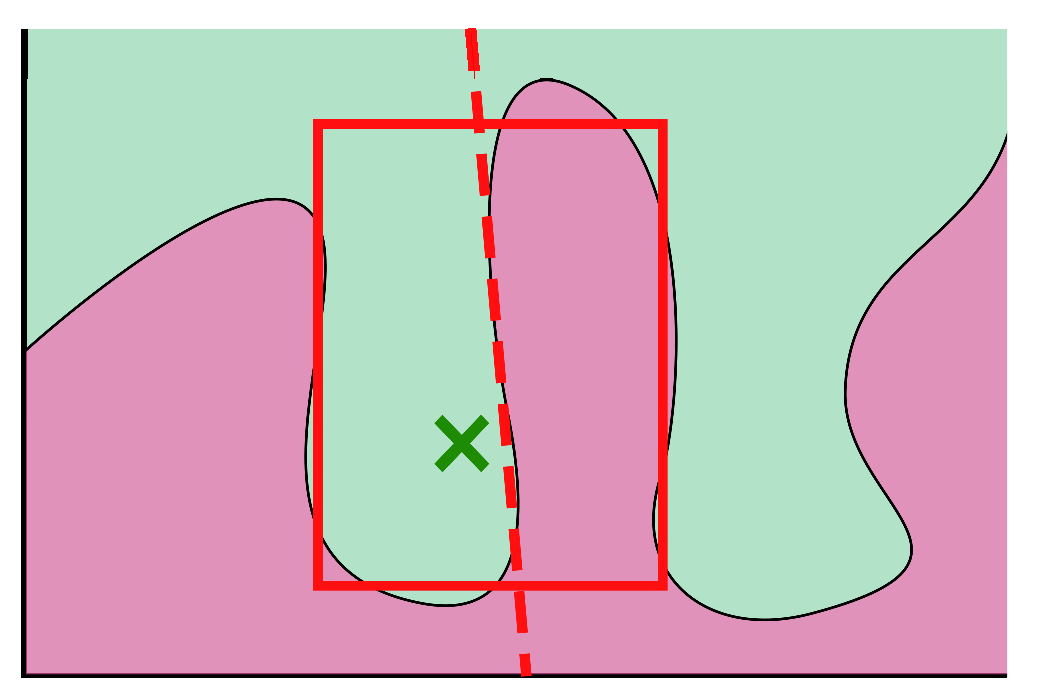
\includegraphics[width=\textwidth]{visual-rlime3}
    \caption{%
      R-LIME\@:
      Maximizes coverage of a rectangular region
      under lower constraints on the accuracy of the linear classifier.
    }\label{fig:rlime}
  \end{subfigure}
  \caption[Visual comparison of LIME, Anchor and R-LIME]{%
    Visual comparison of LIME, Anchor and R-LIME (our method).
    The dashed line represents the local linear approximation model,
    and the solid line represents the rectangular region containing the focal point.
  }
\end{figure}

\subsection{Previous Work}
We specifically focus on \emph{local} and \emph{model-agnostic} methods.
In this section,
we briefly review existing research on local model-agnostic explanations,
particularly focusing on studies closely related to our proposed method.

\subsubsection[LIME]{%
  LIME (Local Interpretable Model-agnostic Explanations)~\cite{ribeiro2016why}
}
LIME locally
approximates a black-box classifier $f: \mathbb{R}^m \to \{0,1\}$
around a focal point $x \in \mathbb{R}^m$
by a linear classifier $g: \mathbb{R}^m \to \{0,1\}$
(\cref{fig:lime}).
The approximation is performed by the following steps:
\begin{enumerate}
  \item Generating a set of perturbed samples $\mathcal{Z}_p$ around $x$
        and the set of pseudo-labels $f(\mathcal{Z}_p) = \{f(z) \mid z \in \mathcal{Z}_p\}$.
        (i) $x$ is converted into a binary vector
        $x'\in{\{0,1\}}^{m'}$,
        (ii) perturbed samples are generated by drawing non-zero elements
        from $x'$ uniformly at random,
        and (iii) the perturbed samples are converted back to the original space.
  \item Learning a linear classifier $g$
        using $\mathcal{Z}_p$ and $f(\mathcal{Z}_p)$
        by minimizing the following loss function:
        \begin{equation}
          \mathcal{L}(f,g,\pi_x)=\sum_{z\in\mathcal{Z}_p}
          \pi_x(z){\left(f(z)-g(z)\right)}^2,
        \end{equation}
        where $\pi_x(z)$ is a weight function designed to be larger for samples
        closer to $x$, typically defined using an exponential kernel.
\end{enumerate}
LIME provides valuable insights into the local behavior of the model
by showing the contribution of each feature to the output $f(x)$.
However, it does not explicitly indicate the region for generating perturbed samples,
making it difficult for users to assess the effective scope of the explanation
~\cite{ribeiro2018anchors}.

\subsubsection[Anchor]{Anchor~\cite{ribeiro2018anchors}}
Anchor maximizes the coverage of a rectangular region
containing the focal point $x$,
expressed as a conjunction of feature predicates (a rule)
as long as the probability of the black-box classifier $f$
outputting $f(x)$ within the region exceeds a given threshold $\tau$
(\cref{fig:anchor}).
It aims to highlight important features
contributing significantly to the output.
For a discrete $m$-dimensional input space $\ispace$,
a trained black-box classifier $f: \ispace \to \{0,1\}$,
an instance $x \in \ispace$
and a distribution $\mathcal{D}$ over the input space,
a rule $A(z) = a_{i_1}(z) \wedge a_{i_2}(z) \wedge \dots \wedge a_{i_t}(z)$ is defined.
The predicate $a_i(z)$ evaluates to true ($=1$) when $z_i = x_i$ and false ($=0$) otherwise.
The reliability of the explanation is defined as the ``accuracy'' of the rule,
and the generality of the explanation is defined as the ``coverage'' of the rule.
The accuracy $\Prec(A)$ and coverage $\Cov(A)$ of the rule $A$ are defined as follows:
\begin{align}
  \Prec(A) & =\mathbb{E}_{z\sim\mathcal{D}(z|A)}
  [\mathbbm{1}_{f(z)=f(x)}], \label{eq:anchor-def-prec} \\
  \Cov(A)  & =\mathbb{E}_{z\sim\mathcal{D}(z)}[A(z)],
\end{align}
where $\mathcal{D}(z|A)$ is the conditional distribution in the region
where the rule $A$ returns true.
$\Prec(A)$ represents the probability that the output of $f$ matches
between the perturbation $z\sim\mathcal{D}(z|A)$ and the focal point $x$,
and $\Cov(A)$ expresses the probability that the perturbation $z$ fits into $A$.
Anchor maximizes coverage as long as
the accuracy of the rule $A$ exceeds a given threshold $\tau$.
However, \cref{eq:anchor-def-prec} is not directly computable.
Introducing a confidence level $1-\delta$ $(0\le\delta\le1)$,
the accuracy constraint is relaxed as follows:
\begin{equation}
  \label{eq:const-prec}
  P(\Prec(A)\ge\tau)\ge1-\delta.
\end{equation}
Thus, the following optimization problem is solved:
\begin{equation}
  \label{eq:main-problem}
  A^*=\underset{A \text{~s.t. } P(\Prec(A)\ge\tau)\ge1-\delta\wedge A(x)=1}
  {\arg\max}\Cov(A).
\end{equation}

\subsection{Overview}
We propose R-LIME,
a method that aims to address the limitations of LIME~\cite{ribeiro2016why}
and Anchor~\cite{ribeiro2018anchors}.
Our method locally approximates the given black-box classifier $f$
around the focal point $x$ by a linear classifier $g$ similar to LIME,
but generates the perturbed samples
from a rectangular region similar to Anchor
so that the generality of approximation is explicitly provided
(\cref{fig:rlime}).

Anchor maximizes the coverage of region $A$
as long as the probability of the output of the black-box classifier $f$ matching $f(x)$
within $A$ exceeds a given threshold $\tau$.
R-LIME, on the other hand, learns a linear classifier $g$
within the rectangular region $A$ and maximizes the coverage of $A$
under lower constraints on the accuracy of $g$.
We modify Anchor's definition of accuracy in \cref{eq:anchor-def-prec}
as follows:
\begin{equation}
  \Prec(A)=\underset{g\in G}{\max}\ \mathbb{E}_{z\sim\mathcal{D}(z|A)}
  [\mathbbm{1}_{f(z)=g(z)}], \label{eq:def-prec}
\end{equation}
where $G$ is a hypothesis space of possible linear classifiers.
By solving the optimization problem in \cref{eq:main-problem}
under the modified definition of accuracy in \cref{eq:def-prec},
we can select the rule that enables explanation with high accuracy and generality.

\subsection{Algorithm}
{%
  \begin{figure}[t]
    \centering
    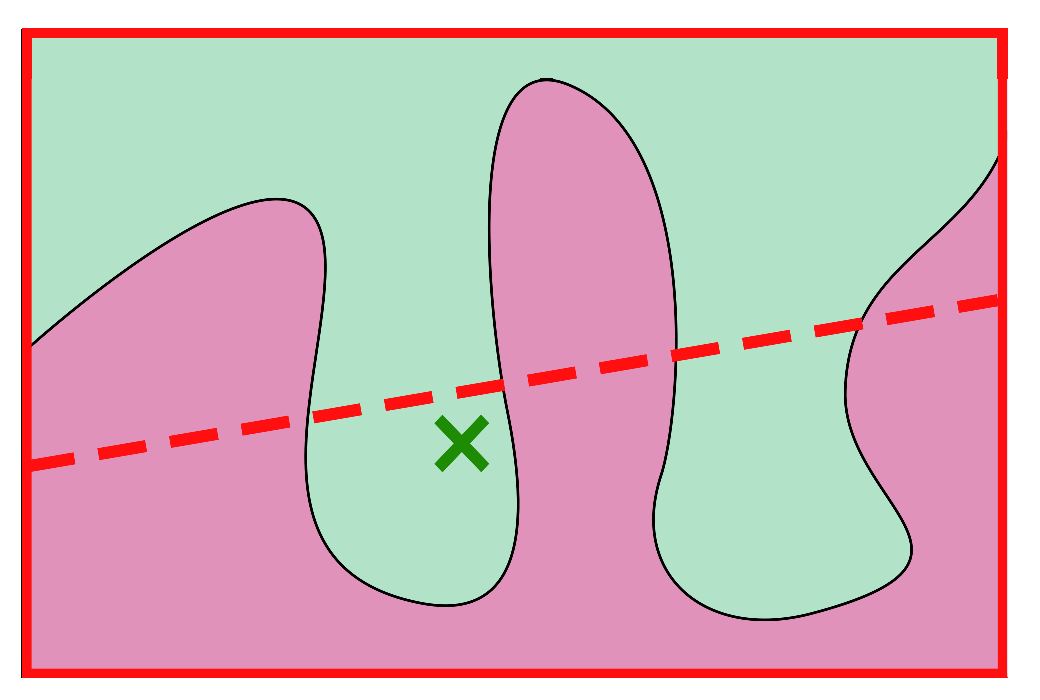
\includegraphics[width=0.32\textwidth]{visual-rlime1}
    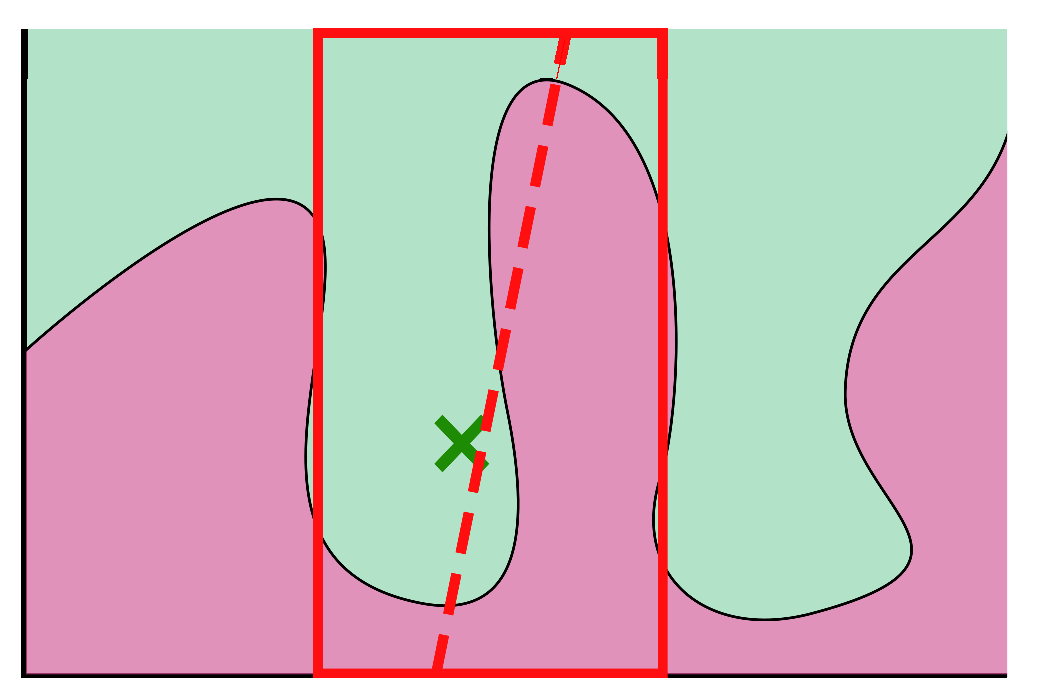
\includegraphics[width=0.32\textwidth]{visual-rlime2}
    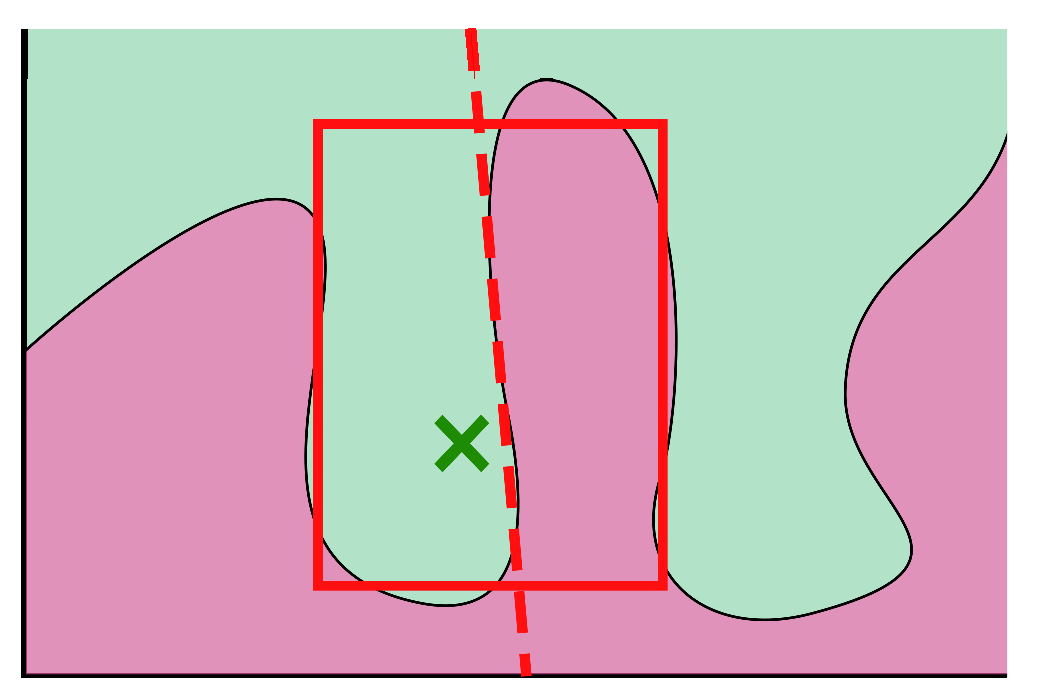
\includegraphics[width=0.32\textwidth]{visual-rlime3}
    \caption[Overview of the R-LIME algorithm]{%
      Overview of the R-LIME algorithm.
      The progression of the algorithm is illustrated from left to right.
      The solid line represents the rectangular region $A$,
      and the dashed line represents the linear approximation model $g$
      learned within $A$.
      The initial value of $A$ is an empty rule (entire input space),
      and predicates are added to $A$, reducing coverage.
      The process continues until $\Prec(A)\ge\tau$ is satisfied,
      at which point the rule with the maximum coverage is output.
    }
  \end{figure}
  \def\myidt{\hspace{\algorithmicindent}}
  \begin{algorithm}[p]
    \small
    \caption{R-LIME}\label{alg:greedy-search}
\begin{algorithmic}[1]
	\Require{%
		Black-box model $f$, Target instance $x$,
		Distribution $\mathcal{D}$,
		Threshold $\tau$, Beam width $B$, Tolerance $\epsilon$,
		Confidence level $1-\delta$
	}
	\Ensure{%
		Rule $A^*$ satisfying Eq.~\eqref{eq:main-problem}
	}
	\State{$A^*\gets\textbf{null},\ \mathcal{A}_0\gets\emptyset,\ t\gets0$}
	% \Comment{%
	%   Initialize the set of candidate rules $\mathcal{A}_0$ to $\emptyset$
	% }
	\Comment{Initialize the set of candidate rules $\mathcal{A}_0$ to $\emptyset$}
	\While{$A^*=\textbf{null}$}
	\State$t\gets t+1$
	\State$\cands_t\gets$ \Call{GenerateCands}
	{$\mathcal{A}_{t-1}$}
	\State$\mathcal{A}_t\gets$ \Call{B-BestCands}
	{$\cands_{t},\mathcal{D},B,\epsilon,\delta$}
	\State$A^*\gets$ \Call{LargestCand}
	{$\mathcal{A}_t,\tau,\delta$}
	\EndWhile%
\end{algorithmic}

  \end{algorithm}

  \begin{algorithm}[p]
    \small
    \caption{Generating new candidate rules}\label{alg:generate-cands}
\begin{algorithmic}[1]
	\Function{GenerateCands}{$\mathcal{A},x$}
	\IIf{$\mathcal{A}=\emptyset$}{\Return{$\{\mathit{true}\}$}}
	\Comment{An initial empty rule always returns $\mathit{true}$}
	\State$\cands\gets\emptyset$
	\ForAll{$A\in\mathcal{A}$}
	\ForAll{$a\in (T(x)\setminus A)$}
	\State$\cands\gets\bar{\mathcal{A}}\cup(A\wedge a)$
	\Comment{Get a new rule by adding a new predicate $a$ to $A$}
	\EndFor%
	\EndFor%
	\State\Return{$\cands$}
	\EndFunction%
\end{algorithmic}

  \end{algorithm}

  \begin{algorithm}[p]
    \small
    \caption{%
	Searching rules with highest accuracy (KL-LUCB~\cite{kaufmann2013information})
}\label{alg:best-cands}
\begin{algorithmic}[1]
	\Function{B-BestCands}{$\cands,\mathcal{D},B,\epsilon,\delta$}
	\State\textbf{initialize} $\Prec,\Prec_{u},\Prec_{l}$ for $\forall A\in\cands$
	\State$\mathcal{A}\gets\Call{B-ProvisionallyBestCands}{\cands}$
	\Comment{$B$ rules with highest accuracy}
	\State$A\gets\arg\min_{A\in\mathcal{A}}\Prec_{l}(A,\delta)$
	\Comment{The rule with the smallest lower bound}
	\State$A'\gets\arg\max_{A'\notin(\cands\setminus\mathcal{A})}\Prec_{u}(A',\delta)$
	\Comment{The rule with the largest upper bound}
	\While{$~\Prec_{u}(A',\delta)-\Prec_{l}(A,\delta)>\epsilon$}
	\State\textbf{sample} $z\sim\mathcal{D}(z|A),z'\sim\mathcal{D}(z'|A')$
	\State\textbf{update} $\Prec,\Prec_{u},\Prec_{l}$ for $A$ and $A'$
	\State$\mathcal{A}\gets\Call{B-ProvisionallyBestCands}{\cands}$
	\State$A\gets\arg\min_{A\in\mathcal{A}}\Prec_{l}(A,\delta)$
	\State$A'\gets\arg\max_{A'\notin(\cands\setminus\mathcal{A})}\Prec_{u}(A',\delta)$
	\EndWhile%
	% \State\algorithmicdo%
	% \State\myidt$\mathcal{A}\gets\Call{B-ProvisionallyBestCands}{\cands}$
	% \State\myidt$A\gets\arg\min_{A\in\mathcal{A}}\Prec_{l}(A)$
	% \State\myidt$A'\gets\arg\max_{A'\notin(\cands\setminus\mathcal{A})}\Prec_{u}(A')$
	% \State\myidt\textbf{sample} $z\sim\mathcal{D}(z|A),z'\sim\mathcal{D}(z'|A')$
	% \State\myidt\textbf{update} $\Prec,\Prec_{u},\Prec_{l}$ for $A$ and $A'$
	% \State\algorithmicwhile$~\Prec_{u}(A')-\Prec_{l}(A)>\epsilon$
	\State\Return{$\mathcal{A}$}
	\EndFunction%
\end{algorithmic}

  \end{algorithm}

  \begin{algorithm}[p]
    \small
    \caption{%
  Searching a rule with highest coverage under constraint
}\label{alg:largest_valid_cand}
\begin{algorithmic}[1]
  \Function{LargestCand}{$\mathcal{A},\tau,\delta$}
  \State$A^*\gets\textbf{null}$
  \Comment{If no rule satisfies the constraint, return $\textbf{null}$}
  \ForAll{$A\in\mathcal{A}$ s.t. $\Prec_{l}(A,\delta)>\tau$}
  \IIf{$\Cov(A)>\Cov(A^*)$}{$A^*\gets A$}
  \EndFor%
  \State\Return{$A^*$}
  \EndFunction%
\end{algorithmic}

  \end{algorithm}
}
The algorithm of R-LIME
is mainly based on that used in Anchor\cite{ribeiro2018anchors}.
For non-convex optimization problems like \cref{eq:main-problem},
greedy search are often used.
But greedy methods tend to converge to local optima,
so we use beam search, which selects multiple candidates at each iteration.
The pseudo-code is shown in \cref{alg:greedy-search}.

\subsubsection{Generating New Candidate Rules}
To generate new candidate rules,
one additional predicate is added to each of the $B$ candidate rules
selected in the previous iteration.
The pseudo-code is shown in \cref{alg:generate-cands}.
$T(x)$ is the set of predicates $\{a_1,\dots,a_m\}$,
where $a_i(z)$ evaluates to true when $z_i=x_i$ and false otherwise.
$T(x)\setminus A$ is the set of predicates in $T(x)$ not included in rule $A$.

\subsubsection{Searching Rules with Highest Accuracy}
Given the set of candidate rules $\cands$,
the algorithm selects the $B$ candidate rules with the highest accuracy.
This problem can be formulated
as best arm identification in the multi-armed bandit framework.
Each candidate rule $A_i\in\cands$ is considered as an arm,
and reward of arm $a_i$ follows a Bernoulli distribution
with $P(X=1)=\Prec(A_i)$.
By sampling $z\sim\mathcal{D}(\cdot|A_i)$
and obtaining the reward $\mathbbm{1}_{f(z)=g_i(z)}$ for each trial,
the algorithm updates $g_i$ using $z$ and $f(z)$ after each trial.
To efficiently search the rule (arm) with the highest accuracy,
we employ KL-LUCB algorithm~\cite{kaufmann2013information}.
The pseudo-code is shown in \cref{alg:best-cands}.
For tolerance $\epsilon\in[0,1]$, KL-LUCB algorithm guarantees below:
\begin{equation}
  P(\underset{A\in\cands}{\min}\Prec(A)\ge
  \underset{A'\in\mathcal{A}}{\min}\Prec(A')-\epsilon)\ge1-\delta.
\end{equation}
However,
KL-LUCB algorithm assumes that the reward distribution for each arm
remains unchanged,
while our method updates the classifier $g_i$ with each sampling,
which may not satisfy the assumption.
This issue is discussed further in \cref{sec:reward}.

\subsubsection{Searching a Rule with Highest Coverage under Constraint}
To satisfy the constraint imposed by \cref{eq:const-prec},
a rule $A$ needs to meet the following condition:
\begin{equation}
  \Prec_{l}(A,\delta)>\tau,\label{eq:stop-condition}
\end{equation}
where $\Prec_{l}(A,\delta)$ is the lower limit of
the $100(1-\delta)$\% confidence interval for $\Prec(A)$.
If the set of candidate rules $\mathcal{A}$
includes rules satisfying \cref{eq:stop-condition},
the one with the maximum coverage among them is selected,
then the iteration is terminated.
If $\mathcal{A}$ does not contain any rule satisfying \cref{eq:stop-condition},
it returns \textbf{null},
and proceeds to the next iteration.
The pseudo-code is presented in \cref{alg:largest-valid-cand}.

% The algorithmic procedure outlined above approximates
% the solution to the optimization problem in \cref{eq:main-problem}
% under the definition of accuracy in \cref{eq:def-prec}. 

\subsection{Computational Complexity}\label{subsec:complexity}
Post-hoc explanation methods including LIME, Anchor, and R-LIME
need to sample a perturbation vector
and get the output of the black-box model multiple times,
which is computationally expensive.
The number of samples required for LIME is $|\mathcal{Z}_p|$,
which is the number of samples designated by the user.
On the other hand,
the expected number of samples required for Anchor and R-LIME is bounded by
$\mathcal{O}[m\cdot\mathcal{O}_{\mathrm{MAB}[B\cdot m,B]}]$,
where $\mathcal{O}_{\mathrm{MAB}[B\cdot m,B]}$
is the expected number of samples
for best arm identification finding the best $B$ arms from $B\cdot m$ arms.
For KL-LUCB algorithm~\cite{kaufmann2013information},
\begin{equation}
  \mathcal{O}_{\mathrm{MAB}[B\cdot m,B]}=
  \mathcal{O}\left[\frac{Bm}{\epsilon^2}\log\frac{Bm}{\epsilon^2\delta}\right].
\end{equation}
Then the total expected number of samples for Anchor and R-LIME is bounded by
\begin{equation}
  \mathcal{O}\left[\frac{Bm^2}{\epsilon^2}\log\frac{Bm}{\epsilon^2\delta}\right].
\end{equation}

For each iteration of KL-LUCB algorithm, R-LIME needs to update
the linear classifier $g_i$, which is not required in Anchor.
If we use logistic regression as the linear classifier and update it
by stochastic gradient descent (SGD)~\cite{robbins1951stochastic},
the computational complexity of updating $g_i$ is $\mathcal{O}(m)$.
It is negligible compared to the complexity of generating a perturbed sample,
which is $\mathcal{O}(m^2)$ if we get a sample
from a multivariate normal distribution using Cholesky decomposition in advance.
Overall, the computational complexity of R-LIME is comparable to that of Anchor.

\section{Experiments}
To verify the effectiveness of our method,
we compared LIME, \hl{Anchor} and R-LIME using a real-world dataset.
\hl{Our code for R-LIME is available on GitHub}\footnote{\url{https://github.com/g-ohara/rlime}}.

\newpage
\subsection{Qualitative Evaluation}\label{sec:exp-qual}
\subsubsection{Experimental Setup}\label{sec:exp-setting}
{%
  \renewcommand{\arraystretch}{1.05}
  \begin{table}[tbp]
    \centering
    \caption[Attributes of the recidivism dataset used in the experiments]{%
      Attributes of the recidivism dataset used in the experiments.
      Continuous features are all discretized,
      and only binary and ordinal features are considered.
    }\label{tab:rcdv}
    \begin{tabular}{llc}
      \toprule
      Attribute              & Overview                              & \# of Possible Values \\
      \midrule
      Race                   & Race (Black or White)                 & 2                     \\
      Alcohol                & Presence of serious alcohol issues    & 2                     \\
      Junky                  & Drug usage                            & 2                     \\
      Supervised Release     & Supervised release                    & 2                     \\
      Married                & Marital status                        & 2                     \\
      Felony                 & Felony or not                         & 2                     \\
      WorkRelease            & Participation in work release program & 2                     \\
      Crime against Property & Crime against property or not         & 2                     \\
      Crime against Person   & Crime against a person or not         & 2                     \\
      Gender                 & Gender (Female or Male)               & 2                     \\
      Priors                 & Number of prior offenses              & 4                     \\
      YearsSchool            & Years of formal education completed   & 4                     \\
      PrisonViolations       & Number of prison rule violations      & 3                     \\
      Age                    & Age                                   & 4                     \\
      MonthsServed           & Months served in prison               & 4                     \\
      \midrule
      Recidivism             & Recidivism or not                     & 2                     \\
      \bottomrule
    \end{tabular}
  \end{table}
}

We used the recidivism dataset~\cite{schmidt1988predicting} for our experiments.
The dataset contains personal information on 9549 prisoners released from
North Carolina prisons between July 1, 1979, and June 30, 1980.
As shown in \cref{tab:rcdv}, the dataset includes 19 items such as
race (\emph{Race}), gender (\emph{Gender}),
presence of alcohol dependence (\emph{Alcohol}),
number of prior offenses (\emph{Priors}),
and presence of recidivism (\emph{Recidivism}).
For this experiment,
we treated the binary classification problem of predicting
the presence of recidivism (\emph{Recidivism}) as the target label.
We discretized continuous features and removed missing values,
resulting in 15 features.

We splitted the dataset into training data (7639 instances) and test data (955 instances),
and trained a random forest model with 50 trees as the black-box classifier
using the training data.
Then, we generate LIME, \hl{Anchor} and R-LIME explanations
for two instances extracted from the test data (\cref{fig:instance}).
For R-LIME, we used logistic regression as the linear approximation model,
and a multivariate normal distribution estimated from the training data
as the distribution $\mathcal{D}$.
\hl{For both Anchor and R-LIME,} the beam width was set to $B=10$,
the confidence coefficient to $1-\delta=0.95$,
and the tolerance of KL-LUCB algorithm to $\epsilon=0.05$.
The accuracy threshold $\tau$ was set to $\tau=0.70,0.90$.

This problem setting can be considered as a case
where a complex machine learning model is introduced to decide parole for prisoners.
Since such decisions can have a significant impact on a person's life,
it is crucial for users to appropriately interpret the outputs of black-box models.
  {%

    \def\dir{src/experiments/exp1/ver1/examples/output}
    \def\Asample{0012}
    \def\Bsample{0011}

    {%
      \renewcommand{\arraystretch}{1.02}
      \begin{figure}[tbp]
        \foreach\a in {0,1}{%
            \centering
            \begin{subfigure}{\textwidth}
              \centering
              \begin{tabular}{p{14em}m{16em}}
                \toprule
                \csvreader[no head, late after line= \\]{%
                  \dir/\sampleindex{\a}.csv
                }{}{%
                \ifnum\thecsvrow=16 \midrule\fi\csvcoli & \csvcolii % chktex 1
                }
                \bottomrule
              \end{tabular}
              \caption{Instance~\AB{\a}}
              \vspace{15pt}
            \end{subfigure}
          }
        \vspace{-15pt}
        \caption[Two instances sampled from recidivism dataset]{%
          Two instances sampled from training data of recidivism dataset.
          Each number in parentheses represents the integer value assigned
          to the corresponding categorical value.
        }\label{fig:instance}
      \end{figure}
    }
  }

  {%
    \def\scale{0.315}
    \def\dir{exp1/ver1/examples/output}
    \def\imgwidth{0.3\textwidth}
    \def\hspacebase{\hspace{-1.5em}}
    \def\vspacebase{\vspace{0.5em}}
    \def\vspacebeforecaption{\vspace{-0.4em}}
    \begin{figure}[t]
      \begin{subfigure}[t]{0.45\textwidth}
        \centering
        \begin{subfigure}[t]{\textwidth}
          \hspace{-10pt}
          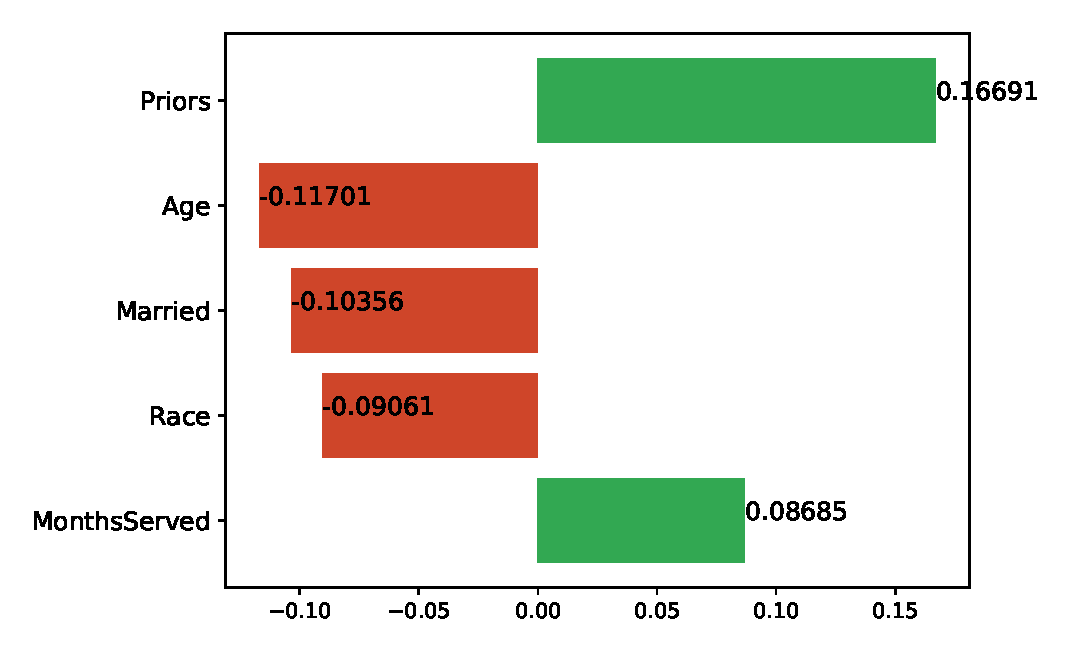
\includegraphics[scale=\scale]{exp1/ver1/examples/output/lime-0012}
          \caption{LIME}\label{fig:lime-0}
          \vspace{1.0em}
        \end{subfigure}

        \vspace{10pt}
        \begin{subfigure}[t]{\textwidth}
          \centering
          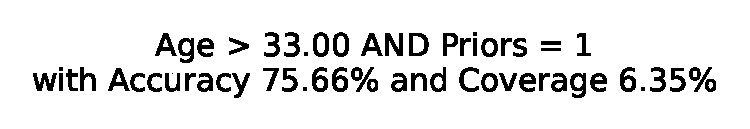
\includegraphics[scale=0.33]{exp1/ver2/examples/anchor-0012-70}  % chktex 8
          \caption{\hl{Anchor ($\tau=0.70$)}}\label{fig:anchor-0-70}
          \vspace{1.0em}
        \end{subfigure}

        \vspace{10pt}
        \begin{subfigure}[t]{\textwidth}
          \centering
          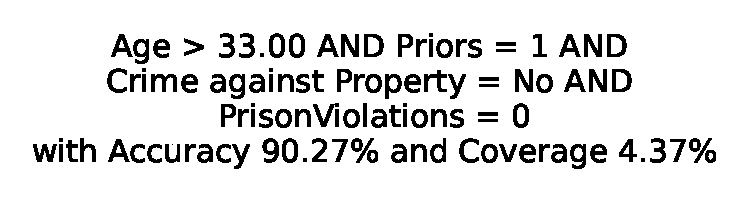
\includegraphics[scale=0.33]{exp1/ver2/examples/anchor-0012-90}  % chktex 8
          \caption{\hl{Anchor ($\tau=0.90$)}}
          \vspace{1.0em}
        \end{subfigure}
      \end{subfigure}
      \hfill
      \begin{subfigure}[t]{0.45\textwidth}
        \begin{subfigure}[t]{\textwidth}
          \hspacebase{}
          \hspace{-5pt}
          \includegraphics[scale=\scale]{exp1/ver1/examples/output/newlime-0012-70}  % chktex 8
          \vspacebeforecaption{}
          \caption{R-LIME ($\tau=0.70$)}\label{fig:rlime-0-70}
          \vspacebase{}
        \end{subfigure}
        \begin{subfigure}[t]{\textwidth}
          \hspacebase{}
          \hspace{-17pt}
          \includegraphics[scale=\scale]{exp1/ver1/examples/output/newlime-0012-90}  % chktex 8
          \vspacebeforecaption{}
          \caption{R-LIME ($\tau=0.90$)}
          \vspacebase{}
        \end{subfigure}
      \end{subfigure}
      \caption[Explanation for Instance A by LIME and R-LIME]{%
        Explanation for Instance A by LIME and R-LIME\@.
      }\label{fig:A}
    \end{figure}
    \begin{figure}[t]
      \begin{subfigure}[t]{0.45\textwidth}
        \begin{subfigure}[t]{\textwidth}
          \hspace{-26.5pt}
          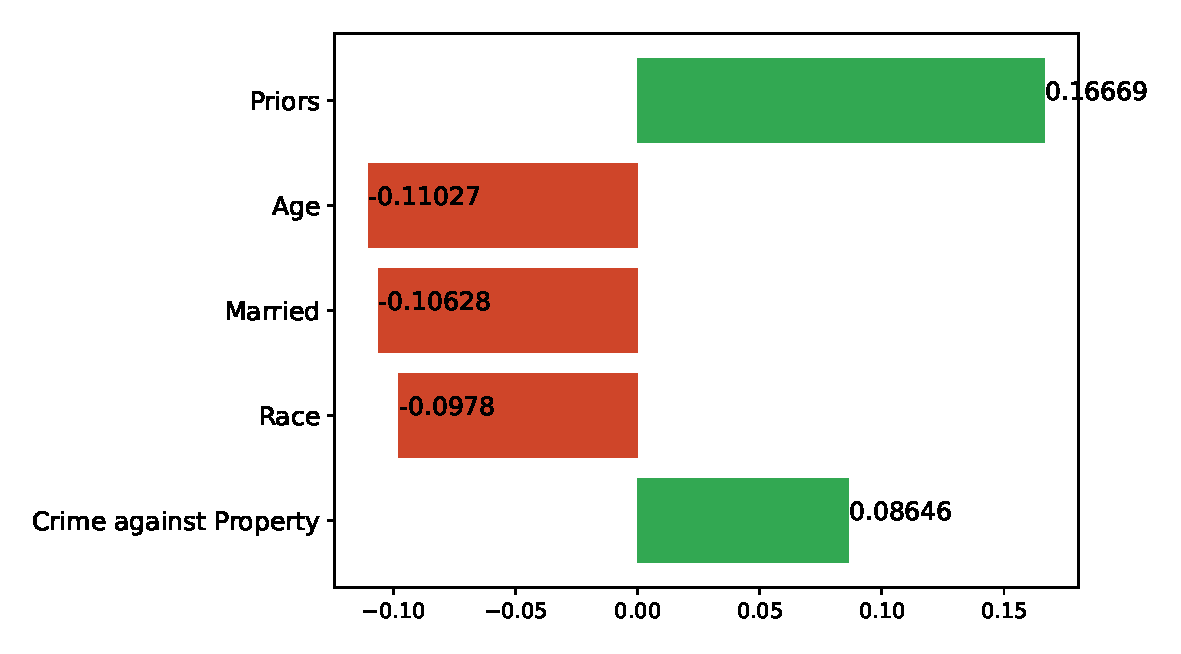
\includegraphics[scale=\scale]{exp1/ver1/examples/output/lime-0011}
          \caption{LIME}\label{fig:lime-1}
          \vspace{1.0em}
        \end{subfigure}

        \vspace{10pt}
        \begin{subfigure}[t]{\textwidth}
          \centering
          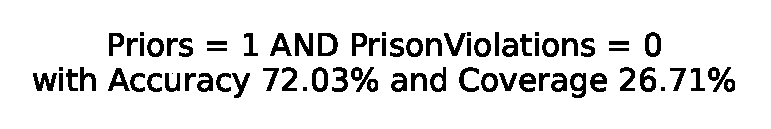
\includegraphics[scale=0.33]{exp1/ver2/examples/anchor-0011-70}  % chktex 8
          \caption{\hl{Anchor ($\tau=0.70$)}}
          \vspace{1.0em}
        \end{subfigure}

        \vspace{10pt}
        \begin{subfigure}[t]{\textwidth}
          \centering
          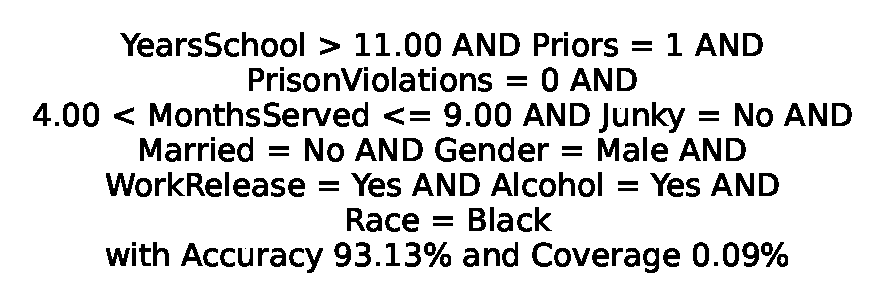
\includegraphics[scale=0.33]{exp1/ver2/examples/anchor-0011-90}  % chktex 8
          \caption{\hl{Anchor ($\tau=0.90$)}}
          \vspace{1.0em}
        \end{subfigure}
      \end{subfigure}
      \hfill
      \begin{subfigure}[t]{0.45\textwidth}
        \begin{subfigure}[t]{\textwidth}
          \hspacebase{}
          \hspace{-5pt}
          \includegraphics[scale=\scale]{exp1/ver1/examples/output/newlime-0011-70}  % chktex 8
          \vspacebeforecaption{}
          \caption{R-LIME ($\tau=0.90$)}
          \vspacebase{}
        \end{subfigure}
        \begin{subfigure}[t]{\textwidth}
          \hspacebase{}
          \hspace{-20pt}
          \includegraphics[scale=\scale]{exp1/ver1/examples/output/newlime-0011-90}  % chktex 8
          \vspacebeforecaption{}
          \caption{R-LIME ($\tau=0.90$)}\label{fig:rlime-1-90}
          \vspacebase{}
        \end{subfigure}
      \end{subfigure}
      \caption[Explanation for Instance B by LIME and R-LIME]{%
        Explanation for Instance B by LIME and R-LIME\@.
      }\label{fig:B}
    \end{figure}
  }

\subsubsection{Experimental Results}
The results of the experiment are shown in \cref{fig:A,fig:B}.
The values assigned to each feature name represent the contribution
(weight of the linear classifier)
to the output of the black-box classifier,
normalized such that the absolute sum is 1.
The figures display the 5 features with the highest absolute contribution.

Explanations generated by LIME (\cref{fig:lime-0,fig:lime-1}) provide insights
that having a prior offenses (\emph{Priors}),
being served for a long time in prison (\emph{Months-Served}),
and committing a crime against property (\emph{Crime against Property})
primarily contribute to the positive prediction
(prediction that the prisoner will be re-arrested).
On the other hand,
being elderly (\emph{Age}), being married (\emph{Married}),
and being of white race (\emph{Race}) contribute to the negative prediction
(prediction that the prisoner will not be re-arrested).
While these LIME explanations provide valuable insights into the behavior of
the black-box model,
they do not explicitly indicate the application scope of the explanations,
leaving users unable to determine to which prisoners the explanations are applicable.

\hl{%
  Anchor provides conditions for the model's output to be fixed with high
  probability.
  For example,
  the explanation for instance A under $\tau=0.70$
} (\cref{fig:anchor-0-70})
\hl{%
  means that the model will predict with 75.66 \% probability
  that the prisoner will commit no more crimes
  when a prisoner is older than 33 and has one prior offense.
  Although it clearly provides the explanation's application scope,
  it does not provide details about how these conditions affect the model's output.
}

In contrast to LIME and Anchor,
R-LIME provides both contribution of each feature to the output and
the application scope of the explanation.
For example, the explanation for instance A
under $\tau=0.70$ (\cref{fig:rlime-0-70}) indicates that it is applicable
only to married prisoner (\emph{Married} $=$\emph{Yes}).
R-LIME explanations also provide their accuracy and coverage,
allowing users to evaluate reliability and generality of the explanations.
For example, the coverage of the explanation for instance B under $\tau=0.90$
(\cref{fig:rlime-1-90}) is 0.01\%,
indicating that the decision boundaries around instance B are complex,
making it challenging to obtain a high-accuracy linear approximation.
This information allows users to discern that
the application scope of this explanation is very narrow, limiting its utility.

\begin{figure}[t]
  \begin{subfigure}[t]{0.48\textwidth}
    \centering
    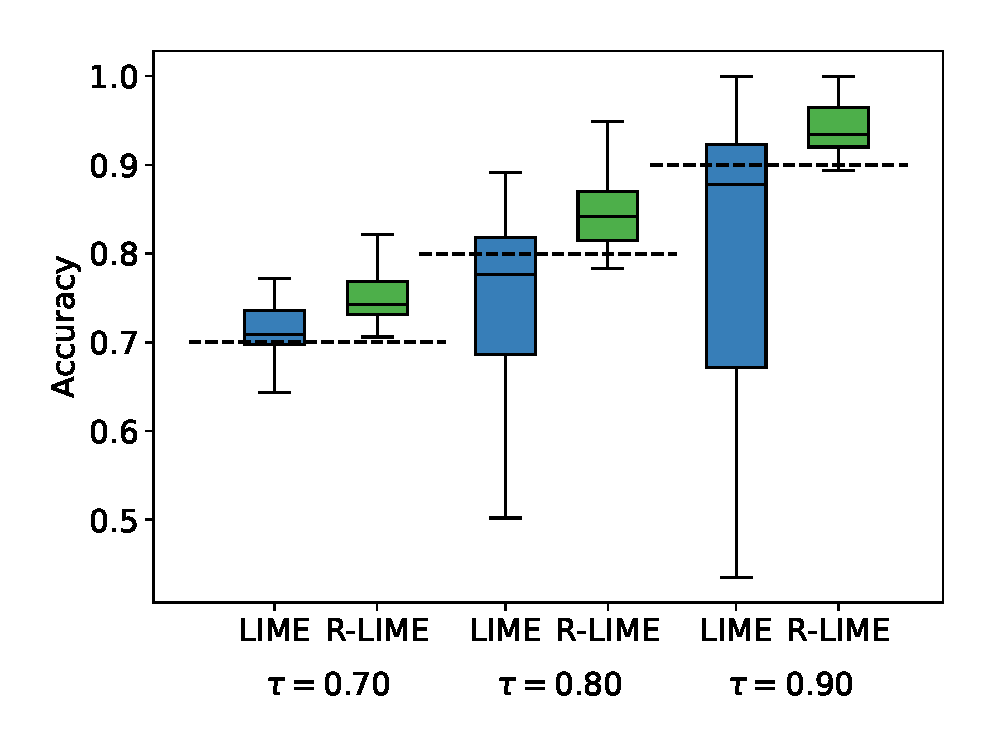
\includegraphics[scale=0.36,valign=t]{exp2/box_plot}
    \caption[Comparison of Local Accuracy between R-LIME and LIME]{%
      Comparison of local accuracy between LIME and R-LIME\@.
      R-LIME achieved higher and less variable accuracy compared to LIME\@.
    }\label{fig:box-plot}
  \end{subfigure}
  \hfill
  \begin{subfigure}[t]{0.48\textwidth}
    \centering
    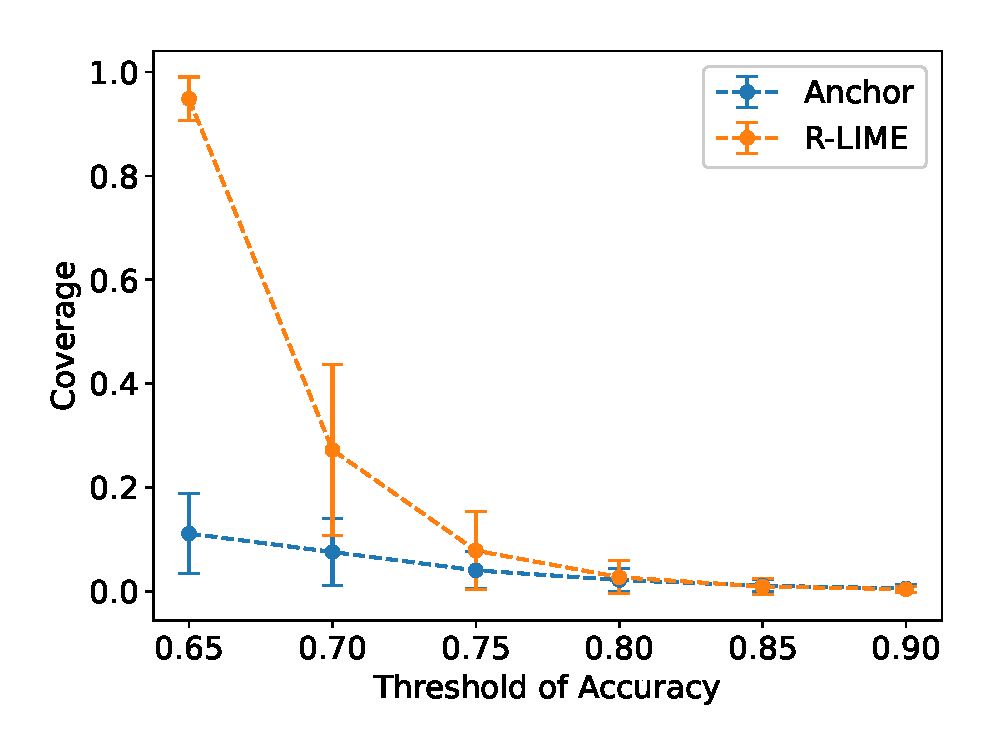
\includegraphics[scale=0.35,valign=t]{exp2b/comp_cov}
    \vspace{3pt}
    \caption[Comparison of Coverage between Anchor and R-LIME]{%
      \hl{%
        Comparison of coverage between Anchor and R-LIME\@.
        R-LIME achieved higher coverage compared to Anchor
        for almost values of $\tau$, especially for relatively small $\tau$.
      }
    }\label{fig:coverage}
  \end{subfigure}
  \caption{Comparison of existing methods (LIME, Anchor) and R-LIME.}
\end{figure}

\vspace{-1pt}
\subsection{Quantitative Evaluation: LIME vs. R-LIME}

\subsubsection{Experimental Setup}
To demonstrate that R-LIME learns a highly accurate linear approximation model
in the optimized approximation region,
we conducted a comparison of the local accuracy of explanations
between LIME and R-LIME\@.
Under the same settings as in \cref{sec:exp-setting},
we randomly sampled 100 instances from the test data of the recidivism dataset
and generated explanations using LIME and R-LIME (with $\tau=0.70,0.80,0.90$).
We then sampled 10,000 instances within the rectangular region
obtained by R-LIME and calculated the local accuracy of both methods.

\subsubsection{Experimental Results}
The results are presented in \cref{fig:box-plot},
showing the distribution of the local accuracy of the linear classifiers
learned by LIME and R-LIME\@.
R-LIME achieved higher accuracy compared to LIME for all values of $\tau$.
This suggests that the linear classifiers learned by LIME and R-LIME
differ significantly,
and R-LIME learns a high-accuracy linear classifier
adapted to the optimized rectangular region.
Additionally, as $\tau$ increases,
the variability in the accuracy of LIME widens.
This indicates that the linear classifiers learned by LIME may not function
effectively as approximation models depending on how the region is selected.

\subsection{\hl{Quantitative Evaluation: Anchor vs. R-LIME}}\label{sec:exp-anchor}
\subsubsection{\hl{Experimental Setup}}
\hl{%
  To demonstrate that R-LIME explanations are more general than Anchor,
  we conducted a comparison of the coverage of explanations
  between Anchor and R-LIME\@.
  Under the same settings as in
}\cref{sec:exp-setting},
\hl{%
  we generated Anchor and R-LIME explanations
  for 100 instances from the test data of the recidivism dataset,
  under the values of $\tau=0.65,0.70,0.75,0.80,0.85,0.90$.
}

\subsubsection{\hl{Experimental Results}}
\hl{The results are presented in} \cref{fig:coverage},
\hl{%
  showing the coverage of the explanations by Anchor and R-LIME\@.
  The coverage of explanations generated by R-LIME is higher compared to Anchor
  for almost values of $\tau$, especially for relatively small $\tau$.
  It is because of the flexibility of the linear approximation models learned by
  R-LIME, which captures the decision boundary more precisely.
  In contrast,
  Anchor uses only the intervals of each feature discretized in advance,
  which cannot capture the decision boundary flexibly and makes its scope narrow.
}


\section{\hl{Discussion}}
 {%
  \def\imgwidth{0.47\textwidth}
  \begin{figure}[t]
    \centering
    \begin{subfigure}[t]{\imgwidth}
      \centering
      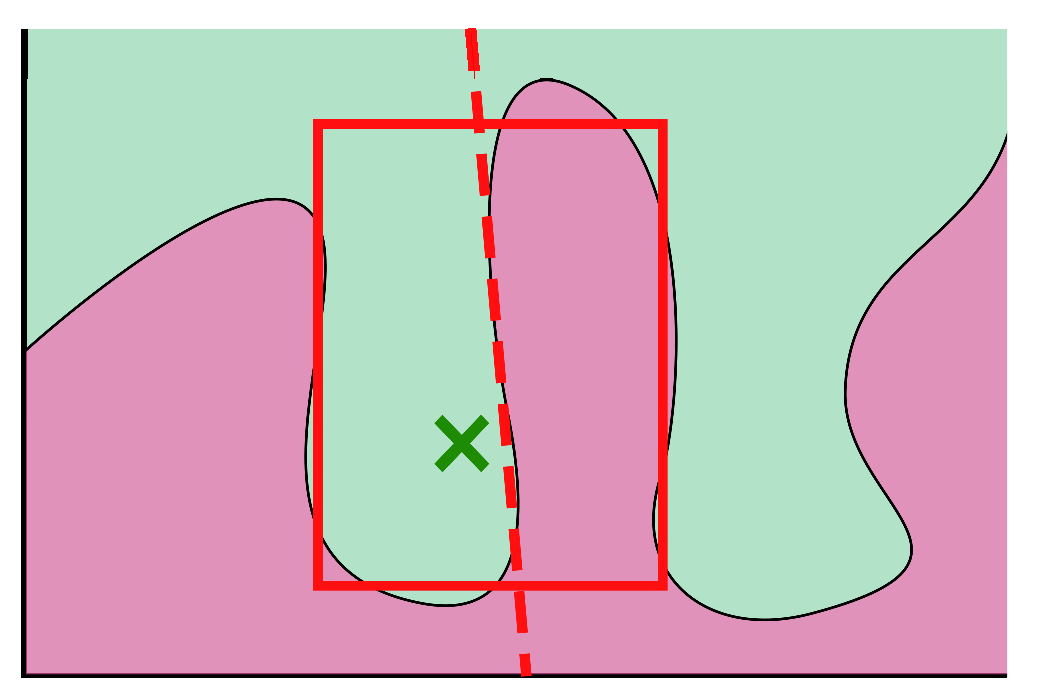
\includegraphics[width=0.7\textwidth]{visual-rlime3}
      \caption{R-LIME for balanced label distribution.}
    \end{subfigure}
    \begin{subfigure}[t]{\imgwidth}
      \centering
      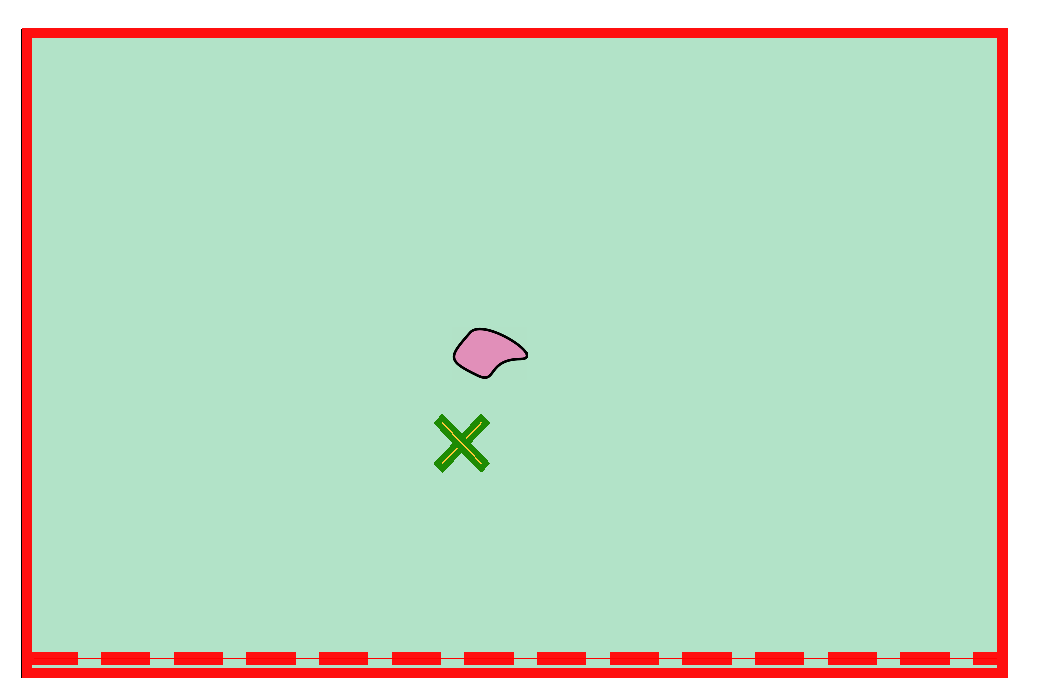
\includegraphics[width=0.7\textwidth]{visual-rlime-imbalanced}
      \caption{R-LIME for imbalanced label distribution.
      }
    \end{subfigure}
    \caption[Behavior of R-LIME for balanced and imbalanced label distribution]{%
      Behavior of R-LIME for balanced and imbalanced label distribution.
      In case of imbalanced label distribution,
      the approximation region covers the entire input space and the
      linear approximation model always outputs the majority label.
    }\label{fig:imbalanced}
  \end{figure}
 }

\subsection{Behavior for Imbalanced Label Distribution}
R-LIME may generate less useful explanations
when the distribution of black-box classifier outputs is imbalanced.
When the ratio of outputting the minority label is less than $1-\tau$,
where $\tau$ is the accuracy threshold,
the approximation region generated by R-LIME covers the entire input space,
and the learned linear classifier always outputs the majority label
(\cref{fig:imbalanced}).

A first possible solution to this problem is modifying the loss function.
Using weighted logistic loss or Focal Loss~\cite{lin2020focal}
as the loss function might lead to the generation of more useful explanations
in the case of imbalanced label distribution.
Another solution involves adding constraints
to limit the label distribution bias within the approximation region.
In addition to \cref{eq:const-prec}, adding a constraint like
\begin{equation}
  {%
    \left(
    \mathbb{E}_{z\sim\mathcal{D}(z\mid A)}[\mathbbm{1}_{f(z)=1}]-\frac{1}{2}
    \right)
  }^2<\mu
\end{equation}
could suppress the excessive expansion of the approximation region.

\subsection{Changes in Reward Distribution in Best Arm Identification}\label{sec:reward}
{%
  \renewcommand{\arraystretch}{1.1}
  \begin{table}[tbp]
    \centering
    \caption[Deviation between the estimated accuracy and the true accuracy]{%
      Deviation between the estimated accuracy and the true accuracy
      of the linear classifier learned by R-LIME\@.
      The deviation $0.012\pm0.017$ was relatively small
      considering the confidence level $1-\delta=0.95$.
    }\label{tab:reward}
    \begin{tabular}{cccc}
  \toprule
                     & Estimated acc. & True acc. & Deviation \\
  \midrule
  Average            & .811           & .829      & .012      \\
  Standard Deviation & .018           & .023      & .017      \\
  \bottomrule
\end{tabular}

  \end{table}
}
For R-LIME,
the problem of selecting the rule with the highest accuracy is formulated
as the best arm identification problem in multi-armed bandit framework,
and solved using KL-LUCB algorithm~\cite{kaufmann2013information}.
However, this algorithm assumes that the reward distribution remains constant,
while in R-LIME,
the reward distribution (accuracy of the linear approximation)
changes with every update of the approximation model after sampling.
Therefore, rewards obtained at an early stage
might influence the estimated value and
make it deviate from the true value.

We conducted an experiment to evaluate the deviation
between the estimated accuracy and the true accuracy.
We generated explanations for 3200 data instances sampled from the dataset,
and compared the estimated accuracy with the true accuracy.
The true accuracy was calculated based on 1000 instances sampled
within the approximation region.
The results in \cref{tab:reward} show a mean deviation of 0.012
with a standard deviation of 0.017.
By considering the confidence level $1-\delta=0.95$,
the deviation was relatively small.
While there are concerns about the theoretical validity of using KL-LUCB algorithm,
our results suggest that the deviation is not significant in practice.

\subsection{\hl{Parameter Selection}}\label{sec:param}

\hl{In} \cref{subsec:complexity},
\hl{%
  we discussed about the computational complexity of R-LIME,
  which depends on some hyperparameters.
  R-LIME requires the hyperparameters to be selected by users,
  such as the threshold of accuracy $\tau$, beam width $B$, tolerance $\epsilon$
  and confidence level $\delta$.
  $B$ should be large and $\epsilon$ and $\delta$ should be small for
  accurate results, as long as the computational cost is acceptable.
  On the other hand, $\tau$ should be carefully selected by users,
  sometimes interactively, considering the tradeoff between
  the accuracy and generality of generated explanation.
}

\section{Conclusion}
Existing methods for
local model-agnostic explanations of black-box classifiers,
such as LIME and Anchor,
have limitations that they cannot achieve interpretability of
both the explanation and its application scope.
To address these challenges,
we proposed R-LIME,
a method that locally and linearly approximates the decision boundary
of a black-box classifier and provides a rectangular approximation region,
which is interpretable for users due to being expressed as a conjunction of feature predicates.
We proposed an algorithm to
maximize coverage of the approximation region
as long as the accuracy of the linear approximation model exceeds a given threshold.
Comparing R-LIME with existing methods on the real-world dataset,
we demonstrated that R-LIME achieves interpretability of both the explanation
and its application scope,
and provides explanations more accurate than LIME and more general than Anchor.
Finally,
we discussed the instability of behavior against imbalanced label distributions,
raised questions about the theoretical validity of using KL-LUCB algorithm,
and hyperparameter tuning in practice.

\newpage
\bibliographystyle{src/style/splncs04}
\bibliography{src/myref/myref}
}

% Reset page number and typeset title
\newpage
\setcounter{page}{1}
\paper{}
\renewcommand{\hl}[1]{#1}
\newpage
\setcounter{page}{1}
\paper{}

\end{document}
